\chapter{Introduction}
\label{intro}

\begin{flushright}
\textit{``The Web as I envisaged it, we have not seen it yet.\\ 
The future is still so much bigger than the past.''\\}
Tim Berners-Lee
\end{flushright}

%Content: Gov Linkedata, Spatial data and visualizations, Evolution of LOD cloud: 2014, 2011, 2007, Percentage of geodata on the LOD Cloud

\section{Context}
\label{sec:context}
The Web is currently in a transition phase from Web of documents to Web of Data. New devices and new ways to use them have emerged and changed user interaction with machines. The ubiquity of the Web also creates an unseen 
abundance of information. Data is flowing onto the Web, created by users, generated by sensors, and stored in ever-growing data farms. Geographic data is widely present on the Web as they are used to locate points of interest. At the same time, with the emergence of Open Data, many governments and local authorities are moving from legacy data stored in their databases
to structured data on the Web. Structured data is already present in the many databases, metadata attached to media, and in the millions of spreadsheets created every day across the world. 

The Web of Linked Data, unlike the Web of hypertext documents, is constructed with documents on the Web with links between arbitrary things described by RDF. Tim Berners-Lee \cite{timld} identifies 4 principles known as ``Linked Data principles'' as follows:
\begin{enumerate}
\item Use URIs as names for things
\item Use HTTP URIs so that people can look up those names.
\item When someone looks up a URI, provide useful information, using the standards (RDF*, SPARQL)
\item Include links to other URIs. so that they can discover more things.
\end{enumerate}
Hence, the URIs are used to identify any kind of object or concept on the Web via the HTTP protocol. Linked Data is continuously evolving, started in 2007 with a dozen of datasets (cf. Figure\ref{fig:lodcloud2007}) to a large data space with thousands of datasets on different topics. From 2011 (see Figure \ref{fig:lodcloud2011})\cite{jentzsch2011} to 2014, the number of datasets have tripled, with a significant growth of nearly $271\%$  \cite{max2014}. The new version of the Linked Open Data Cloud in April 2014 contains 1014 linked datasets which are connected by 2909 linksets, as depicted in Figure \ref{fig:lodcloud2014}\footnote{A more Web friendly version can be accessed at \url{http://data.dws.informatik.uni-mannheim.de/lodcloud/2014/}}. In order to enable
Linked Data applications to discover datasets and to ease the integration of data from multiple sources, Linked Data publishers should comply with the following set of best practices for publishing datasets on the Web \cite{Heath2011}:

\begin{itemize}
%\item \todo{add here part of BP doc of GLD group}
\item \textbf{Data selection:} The dataset should be selected based on its potential relevance to be reused in an open format accessible somewhere on the Web.
\item \textbf{Vocabulary usage:} The publishers should use terms from widely-used vocabularies in order to ease the interpretation of their data. If data providers use their own vocabularies, the terms of such proprietary vocabularies should be mapped to existing terms in ``popular'' vocabularies.

\item \textbf{Linking:} By setting RDF links, data providers connect their datasets into a single global data graph which can be navigated by applications. Thus enables the discovery of additional data by following RDF links.

\item \textbf{Dereferencable URIs:} By using HTTP URIs as identifiers for each resource, agents can easily look-up at the resources and ``dereference'' a URI in order to have access to the full representation identified by that URI. This helps build a network of URIs on the Web which enables navigation on different graphs. 

\item \textbf{Metadata provision and machine access to data:} Provide various ways for search engines and other automated processes to access data using standard Web mechanisms.
\end{itemize}

\begin{figure}[ht!]
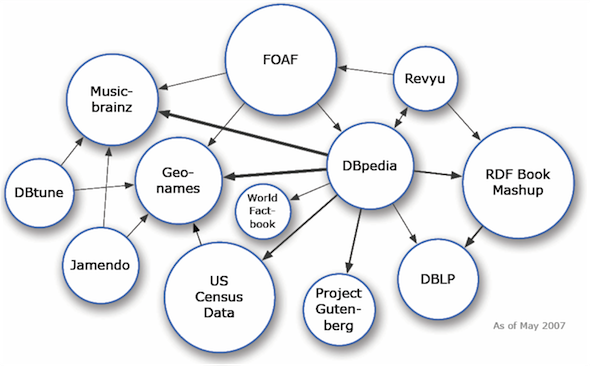
\includegraphics[width=0.9\textwidth]{img/lod-cloud2007.png}
\caption{The LOD cloud as of May, 2007}
\label{fig:lodcloud2007}
\end{figure}

 
However, geospatial data on the Web still lacks of interoperability for a better integration due to these three main factors:
\begin{enumerate}
\item Vendor specific geometry support, such as Google Maps API, Yahoo Geo Technologies, etc.
\item Different vocabularies, such as W3C Basic Geo\footnote{\url{http://www.w3.org/2003/01/geo/}}, NeoGeo\footnote{\url{http://geovocab.org/doc/neogeo/}}, GeoSPARQL  \cite{ogc2012}, GML XMLLiteral\footnote{\url{http://www.opengeospatial.org/standards/gml}} and vendor-specific.
\item Different spatial reference systems, such as Lambert93, WGS84, British National Grid, etc.
\end{enumerate}


The potential of Linked Data for easing the access to government data is increasingly understood, as many countries such as UK, France, Australia, U.S.A. are releasing a significant amount of governmental and public sector data made accessible on the Web. Those organizations and public bodies are moving from legacy data stored in their databases to structured data on the Web. Structured data is already present in many databases, metadata attached to medias, and in the millions of spreadsheets created everyday across the world. However, the full potential of reusing such datasets will happen if they are published on the Web as Linked Data for more discovery and common understanding with appropriate semantically annotations.

\subsection{Geographic Information (GI)}
\label{sec:geoinfo}

Geographic information (GI) surrounds us in our daily life. GI is commonly used to answer questions containing a \textit{where} component. For example in ``where shall Emmy study next year?'', the answer can show the different forms of expressing the location:

\begin{itemize}
\item In the answer: `` Emmy will study in Nice'', Nice is used to identify the global area (locality) of where Emmy will study. In GI, this is an indirect reference. A map can display the geometry, and in the case of ambiguity, more context should be given, such as the country or the region.  
 \item In the answer ``Emmy will study in Sophia-Antipolis, Nice''; there is a relation ``part-Of'' (mereology) between Sophia-Antipolis and Nice, with more precision about the location of where Emmy will study.
 \item In the answer, ``Emmy will study at Eurecom, sophia-Antipolis, Nice'', Eurecom is the building ``within'' (topology)
 \item In the answer, ``Emmy will study at 450, route des Chappes, 06160 Biot, Nice, France'', the full address in provided with  standardized form of addressing, including a post code or zip code.
\end{itemize}
  
Table \ref{tab:address-fr} shows the standard convention used to describe address in France. 

\begin{table}[!htbp]
\centering{
\begin{tabular}{lll}
 \specialrule{1pt}{1pt}{1pt}
 \textbf{Format}	 	& {\textbf{Example}}  \\ \specialrule{1pt}{1pt}{1pt}
\textit{Addressee (Natural person/Organization)} & EURECOM\\
\textit{More detailed description of addressee (optional)} & M. Frank Bender\\
\textit{Housenumber + Streetname} & 450 route des Chappes \\
\textit{Postal code + uppercase town} & 06410 Biot \\
\textit{Country (if other than France)} & \\
 \specialrule{1pt}{1pt}{1pt}
\end{tabular}
\caption{Format of an address in France with the example of EURECOM.}
\label{tab:address-fr}
}
\end{table}

In \cite{ldgeob2013}, the authors summarized clearly the different forms of GI:
\begin{itemize}
\item Geometry: Geometries for GI can use raster or vector representations. In the former, GI is represented as an array of pixels  (or cells), with each cell corresponding to a value and the position of each pixel corresponding to an area in the Earth. The latter is usually represented as a vector data of points, lines and polygones. This representation of GI is the mostly used by geographic datasets in the Web of Data
\item  Topology and Mereology: They are used to model GI topologically and mereologically. Topology expresses the spatial relationships that exist between different objects, and mereology describes the whole-part relationships.
\item  Textual representations, where GI is described as text or directions. Classifications, taxonomies and ontologies are often used to classify objects or geographic features. In this thesis, we use ontologies to describe French features in the French mapping agency.
\end{itemize}
	 
In traditional GI, maps are the most obvious manner to visualize locations. A map is a two-dimensional representation of the landscape that can be used to navigate, visualize different aspects of a feature (street-view, satellite view, etc.).  

\subsection{Geographic Data in the Linked Data Cloud}
\label{sec:geoldcloud}

The Linked Data Cloud originating from the Linking Open Data project classifies the data sets by domains, highlighting the diversity of data sets present in the Web of Data. The last classification in 2014 reveals 8 domains: government, publications, life scences, user-generated content, cross-domain, media, geographic and social Web. 
Geography information is often used to connect information from varied topical domains. This appears in the Web of Data, where the Geonames\footnote{url{http://www.geonames.org/}} dataset serves as a hub for other datasets that have some geospatial component. Geonames is an open-license geographical database that publishes Linked Data about 8 million locations.

\begin{figure}[ht!]
\centering{
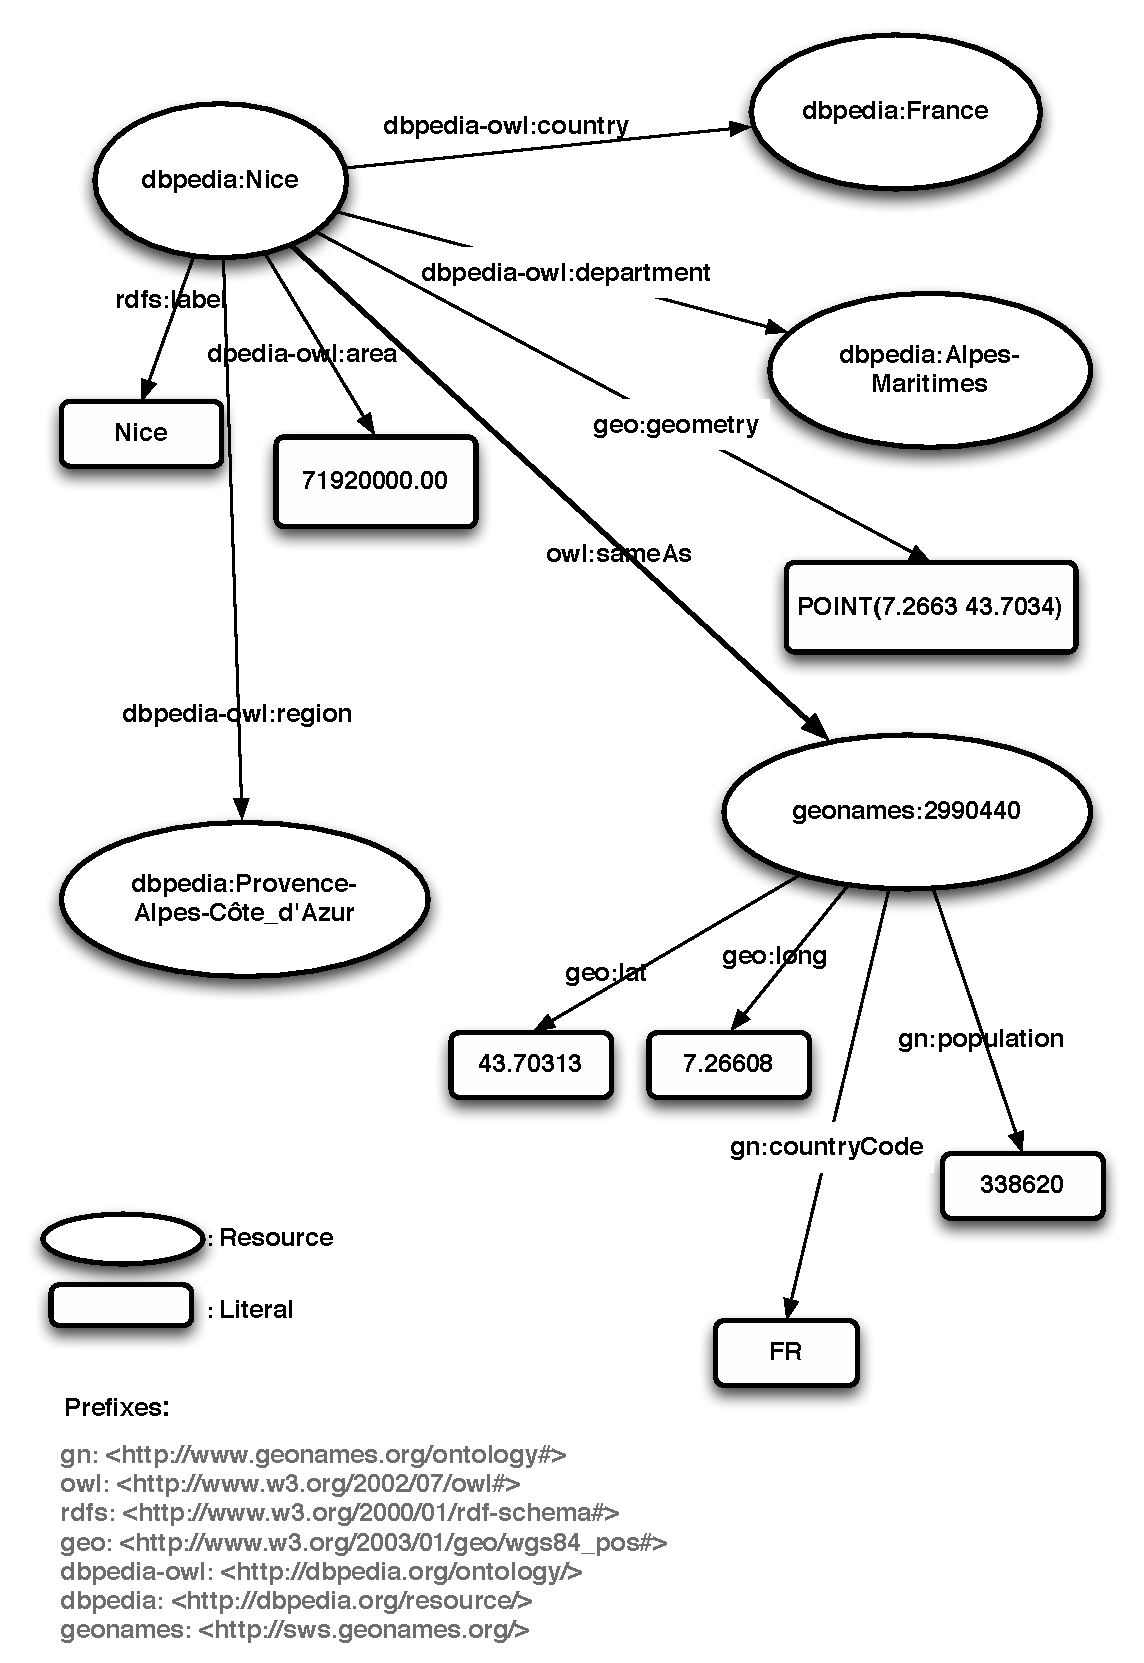
\includegraphics[scale=0.6]{img/nice-resource.pdf}
\caption{RDF representation of the resource of Nice in DBpedia and Geonames}
\label{fig:nice-rdf}
}
\end{figure}

Figure \ref{fig:nice-rdf} depicts a graph model of the city of NICE in France, starting from DBpedia \cite{dbpedia2009} dataset and linked to Geonames with the relation ``owl:sameAs''. In Geonames, the resource is linked back to DBpedia with a different relation, which is ``rdfs:seeAlso''. These different connectors are useful to link different datasets and to achieve the fourth principle of Linked Data as set out by Berners-Lee \cite{timld}:\textit{``include links to other URIs so that they can discover more things''}. 

Another significant dataset in geospatial data is LinkedGeoData \cite{linkedgeodata}, a Linked Data conversion of data from the OpenStreetMap project, which provided information about more than 350 million spatial features. Wherever possible, locations in Geonames and LinkedGeoData are interlinked with corresponding locations in DBpedia, ensuring there is a core of interlinked data about geographical locations.

Ordnance Survey (the national mapping agency of Great Britain) is one of the first mapping agency to publish Linked Data describing the administrative areas within the Great Britain \cite{Goodwin2008}, in efforts related to the \url{data.gov.uk} initiative. Since then, other initiative have begun to publish Linked Data, such as GeoLinkedData(es) \cite{deLeon2010}, Linked Sensor Data, US Census data. 

One of the key benefit of Linked Data is the use of the  RDF model to manipulate data on the Web, interconnect it with other data and consume it in a variety of applications. In the process of getting those datasets effectively published, there are some barriers that prevent publishers to embrace the movement, such as the following:
\begin{itemize}
\item RDF and its different serializations is difficult to understand and use in practice compare to CSV or JSON.
\item Given a dataset, choosing a suitable vocabulary to model the data is a big challenge.
\item There are few easy-to-use tools that guide publishers in their process of publishing their dataset without being specialists in the different technologies: such as SPARQL, server configurations for dereferencing URIs, etc.
\item The tools for converting data into RDF are either more domain-specific, or difficult to configure for non experts.
\end{itemize}

Nevertheless, the resulting ``Web of Data'' has started being populated in different domains, particularly with geospatial data, as proved by the efforts in \cite{goodwin08,linkedgeodata,deLeon2010,Salas2011}. Those efforts and initiatives follow the vision of the \textit{Semantic Geospatial Web} promotes by Max Egenhofer in \cite{egenhofer12} challenging GIS researchers to contribute to the Semantic Web effort by creating geospatial ontologies, query languages and processing techniques adapted to geospatial information on the Web. 


The recent emergence of Linked Data radically changes the way structured data is being considered. By giving standard formats for the publication and interconnection of structured data, linked data transforms the Web into a giant database. While making data available on the Web, there is a need to build meaningful applications to show the value of all the data so that users can easily explore it, and derive new insights from it. As many information visualization (InfoVis) tools are already present in InfoVis community\footnote{\url{http://en.wikipedia.org/wiki/Information_visualization}}, their easy adoption and usage for displaying structured data raise new challenges. Those challenges are the following:
\begin{enumerate}
\item How to specify and define semantic Web applications in terms of tools, widgets that can easily visualize RDF datasets?
\item How to mine efficiently heterogeneous structured data to derive patterns for automatically recommending adequate visualization tool to help users building innovative applications in an affordable time.
\item How could we bridge the gap between traditional infoVis tools and Semantic Web technologies to built easily applications on top of datasets published as L(O)D?
\item How to represent and share visualizations built with datasets already present in different Open Data portals, such as \url{http://data.gouv.fr} and \url{http://data.gov.uk}.  
\end{enumerate}

  

\begin{figure}[ht!]
\centering{
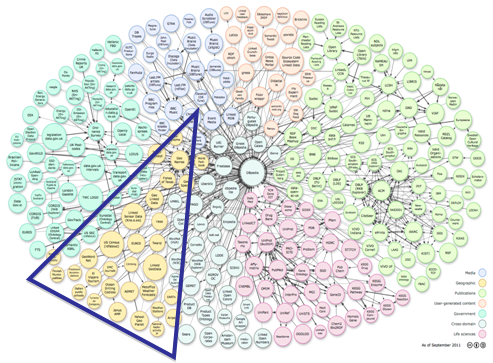
\includegraphics[scale=0.9]{img/lod-diagram-2011.png}
\caption{Linking Open Data cloud diagram 2011, by Anja Jentzsch and Richard Cyganiak. \url{http://lod-cloud.net/.} The highlighted portion corresponds to the geospatial datasets.}
\label{fig:lodcloud2011}
}
\end{figure}


\begin{figure}[ht!]
\centering{
\includegraphics[scale=0.1]{img/LODcloud2014.pdf}
\caption{Linking Open Data cloud diagram 2014, by Max Schmachtenberg, Christian Bizer, Anja Jentzsch and Richard Cyganiak. \url{http://lod-cloud.net/}}
\label{fig:lodcloud2014}
}
\end{figure}



\section{Research Questions}
\label{sec:questions}
 

The ubiquity of the Web is creating an unseen abundance of information. Data is flowing onto the Web, created by users, generated by sensors, and stored in ever growing data farms. Geographic data is widely present on the Web as they are used for location of Point of Interest. At the same time, many organizations are moving from legacy data stored in their databases to structured data on the Web. Structured data is already present in many databases, metadata attached to medias, and in the millions of spreadsheets created everyday across the world. 
Many Linked Open Datasets have geospatial components, but still not having a common ways to describe features, spatial objects or geometries. Given the following three use-cases to express how challenging is to integrate geographic data from different datasets to obtain relevant answers: 
\begin{verbatim}
UC1: What DBpedia Historic Buildings are within walking distance 
     from my current location ?
UC2: What departments are located inside the bounding box 
     composed of the Eurecom location and the Eiffel Tower? 
UC3: Give me the centroids of the administrative units 
     in France in the projection Lambert93?

\end{verbatim} 

 The aforementioned use-cases take into account ``Concepts'' (e.g: Historic Building, Department) that are defined differently depending on the provider of the dataset (e.g: DBpedia, OpenStreetMap, IGN).Further, the aforementioned use-cases implicitly make use of some specific topological functions widely used in the GIS applications, such as ``within'' , ``inside'', ``bounding box''. For example, Use Case 2 also mentioned Lambert93, a specific projection of data in France. Our aim is to contribute to actual efforts in representing geographic objects to leverage the barrier of integration of geospatial data both by the publishers and the lay users consuming the data. 

Our main concern is to tackle the problems within the workflow of publication in two directions, more likely to happen at the beginning and the end: 
\begin{itemize}
\item (i) Geographic Information on the Web of Data: as an application of the life-cycle of publishing geodata.
\item (ii) Visualization tools for building innovative applications consuming structured data: as for leveraging the process of creating applications on-top of semantic data to highlight some relevant knowledge to the users.

\end{itemize}

In \cite{koubarakis12}, the authors mentioned many research topics in the area of linked geospatial data. In this thesis, we address the following challenges:

\begin{enumerate}

\item \textit{Vocabularies:} How do we model geospatial information on the Web? How do we assess geospatial ontologies? How should complex geometry be serialized? 
\item \textit{Query languages:} How do we write efficient queries that target geospatial Web? How do we store and index geodata in RDF ?
\item \textit{Datasets:} How do we extract and convert geodata to expose it on the Web? What are the best practices for representing complex geometries on the Web? How can we integrate fully compatibility of Coordinate Reference Systems (CRSs) on datasets? 
\item \textit{Publication:} How can we develop scalable frameworks for covering the workflow of publishing geodata? What are the appropriate triple stores for handling geodata? What are the metrics to use for interconnecting different geodata resources on the Web?  
\item \textit{Applications and user interfaces:} How do we generate visualizations of linked geospatial data? What are appropriate high-level APIs that ease the development of user interfaces for geospatial data? Can we rely on existing map platforms such as Google Maps, Bing Maps or OpenSteetMap?
\end{enumerate}

In this thesis, we tackle the issues and challenges both from publishers and users point of view. Publishers and users need pragmatic solutions that help them to choose a vocabulary, find a tool to convert ShapeFiles according to well-known vocabularies, then generate and publish the data following some best practices.


After the publication of the dataset using Linked Data paradigm, the logical question is: ``What next''? Publishers and users need to be able to understand their dataset while developers have to build application out of the datasets. There is a huge amount of structured data on the Web, with the expectation to have more and more 
data to be published as LOD. This huge amount of ``structured big data'' is far to reach non-expert users 
so far, due to the complexity of different technologies used to model and query the data. Thus, it is 
important to create visualizations on top of the generated datasets to explore, analyze and showcase 
some of the potential of linked data to non-expert users. In this process, some challenging research questions have to be addressed, such as the following:

\begin{itemize}
\item  How to find suitable visualizations according to the datasets without showing the complexity of SPARQL queries?
 \item  What are the important properties to visualize for entities, depending on the domain and the users' expectations?
 \item  How to bridge the gap between existing traditional tools of Information Visualization, mostly using CSV/XLS, JSON or proprietary formats to easily integrate RDF models as input?
 \item How to make interoperable applications built on top of Government Open Data catalogues? How to reuse existing applications?
\end{itemize}
 
 While trying to answer to the aforementioned challenges, we report the state of the art and related approaches dealing with visualizations for Linked Data. 


\section{Contributions}
\label{sec:contributions}
In this section, we provide the main contributions of this thesis organized in three main parts of our thesis: model and publication of geospatial data, visualizations of data and applications on the Web and contribution to standards. 

\subsection{Modeling, publishing and querying geodata}
The geolocation is crucial for many applications for both human and software agents. More and more data is opened and interlinked using the Linked Data principles, and it is worth modeling geographic data efficiently by reusing as much as possible from existing ontologies or vocabularies that describe both the geospatial features and their shapes. In the first part of our work, we survey different modeling approaches used by the Geographic Information System (GIS) and the Linked Open Data (LOD) communities. Our aim is to contribute to the actual efforts in representing geographic objects with attributes such as location, points of interest (POI), and addresses on the Web of Data. We focus on the French territory and we provide examples of representative vocabularies that can be used for describing geographic objects. We propose some alignments between various vocabularies (DBpedia, GeoNames, Schema.org, LinkedGeoData, Foursquare, etc.) in order to enable interoperability while interconnecting French geodata with other datasets. 

Regarding this aspect of our research, we have achieved the following tasks:
 \begin{enumerate}
 
  \item We have proposed an ontology describing features and points of interest for the French territory, by reusing an existing taxonomy (GeOnto) and aligning it to other related vocabularies in the geolocation domain (Section \ref{sec:bpgeo}).
  \item  We have studied how to extend the existing vocabularies for geographic domain to take into account efficient modeling of complex geometries. By doing so, we tackle the complex geometry representation issues in the Web of Data, describing the state of implementations of geospatial functions in triple stores and comparing them to the new GeoSPARQL standard (Section \ref{sec:specgeosparql}).  We finally make some recommendations and advocate for the reuse of more structured vocabularies for publishing topographic entities to better address the IGN-France requirements. (Section \ref{sec:topofunc}).
  
 \item We have made a comparative study of triple stores, comparing their capability to store spatial information and their implementation of topological functions with respect to the ones 
existing in Open Geospatial Consorcium\footnote{\url{http://www.opengeospatial.org/}} standards (Section \ref{sec:surveytps}).
 \item  We have designed and implemented vocabularies for describing complex geometries with different coordinate systems, with direct application to the French administrative units (Section \ref{sec:geomfeaturevocab}).
 
 \item We have interlinked French authoritative geodata resources with existing geospatial datasets on the Web, such as LinkedGeodata, GADM, NUTS and Geonames (Section \ref{sec:mapping}).
 
 \item We have contributed to the creation of a French LOD Cloud by publishing 8 datasets representing 340 million triples as LOD covering the French territory (Section \ref{sec:frenchCloud}).
 

\end{enumerate}


Consuming data on the Web through visualizations is as challenging as applications have to deal with the graph structure of RDF, the underlying semantics of the dataset and the user interaction to easily understand what the data is about. In the following section, we present our contributions on visualization.
\subsection{Visualization Tools in Linked Government Data} \label{visu}

We first review some innovative applications that have been developed on top of datasets released as Open Data by governments (UK, USA, France) and local authorities. We have then derived and proposed 8 use cases (UCs) that can be developed to consume data from the different main providers in the French level: INSEE, DILA, IGN, FING, etc. We mention that the most interesting use cases are the ones which show the added value of having interconnected datasets. These UCs,  developed and deployed, can be useful to show the benefits of Linked Data in a variety of domains such as education, tourism, cultural heritage, civil administrations, judicial courts, medicine, etc. 

Regarding tools used for visualization, we have identified and classified them in two categories, providing for each of them relevant examples: (i)-tools that operate over RDF data, (ii) and tools that operate over other structured formats. We then provide some basic criteria for assessing a given visualization tool, with some weight attached to each of the criterion. 

Moreover, regarding visualizations on top of datasets, we have contributed as follows:
\begin{enumerate}


\item We have built an application of the French first-round elections in 2012 using data from the \url{http://data.gouv.fr} and other public institutions. The application available at \url{http://www.eurecom.fr/~atemezin/DemoElection/} was built with the Exhibit Framework \cite{exhibit2007}; it aims to showcase the reconciliation of heterogeneous datasets: political results in CSV, unemployment rate, data of candidates, departments of France and more data from DBpedia. The user can filter by candidate image, unemployment rate and department to see the scores, with more enriched information about the department.
 
\item We have implemented a generic tool for exploring geodata on a map, based on the automatic detecting of SPARQL endpoints in the LOD cloud containing geospatial datasets (Section \ref{sec:geordfviz}). 

\item We have implemented an application consuming geodata and statistics combining multiple datasets in education from \url{http://data.gouv.fr} portal (Section \ref{sec:perfectSchool}).

\item we have built an application for conference events (Section \ref{sec:confomaton}) with their associated media reconciled from many social platforms (Instagram, Twitter, etc.).

\item We have built a vocabulary for structuring applications on the Web of Data. The vocabulary can be used for discovering visual tools or charts used to build applications (Section \ref{sec:dvia}). 

\item We have implemented a generic plugin for annotating applications developed for contests to be included in any web page, leveraging  the generation of structured content out of webpages using the vocabulary. 


\item We have implemented a wizard that analyses an RDF dataset and recommend visualization based on predefined categories, using generic SPARQL queries for easing the exploration of datasets published as LOD. 


\end{enumerate}

\subsection{Contributions to Standards}
\label{sec:contrib-standard}
We contributed to the W3C Government Linked Data Working Group (GLD WG)\footnote{http://www.w3.org/2011/gld/} activity from July 2011 until December 2013.  The objective of the Working Group was to \textit{``provide standards and other information which help governments around the world publish their data as effective and usable Linked Data using Semantic Web technologies''}.

We contributed to three task forces as follows:
\begin{itemize}
\item Task Force \#1 aims to create a linked data community directory\footnote{http://dir.w3.org} and to maintain it on-line. The directory covers deployments, vendors, contractors, end-user applications. We contributed to define the requirements and providing data for the French organizations in the directory.

\item Task Force \#2 aims at providing best Practices for publishing Linked Data by producing recommendations regarding vocabulary selection, URI construction, a Linked Data Cookbook, versioning, stability and provenance. Here, we have prepared a checklist to help government to select and re-use vocabularies in their project. We have also proposed our vision of the Linked Open Data Life cycle, with best practices for creating URIs. We served as editor for the Linked Data Glossary \cite{glossairegld} published as a W3C Note document, apart from contributing in many sections of the document ``Best Practices for Publishing Linked Data'' \cite{bpgld}.

\item \textbf{Task Force \#3} goal was to provide relevant vocabularies to be used by governments or local authorities in their process of exposing their data. We have participated actively in the discussions on the different vocabularies published as recommendations by the W3C such as the Data Cube \cite{dcube}, the ORG vocabulary \cite{org} and the DCAT \cite{dcat} vocabulary.
\end{itemize}

Regarding the use of standard vocabularies we have contributed on: 
\begin{itemize}

\item  Proposing a method to harmonize prefixes on the Web of Data  with two services: Linked Open Vocabularies (LOV)\footnote{\url{http://lov.okfn.org/dataset/lov/}} and prefix.cc\footnote{\url{http://prefix.cc}}. The former is currently a maintained hub of curated vocabularies on the Web, while the latter is a focal point for developer to register and look-up prefixes for their resources or ontologies. The approach proposed can be extended to any catalogue of vocabulary as long as the vocabularies fulfill the requirements to be inserted into LOV catalogue (Section \ref{sec:prefharmoni}). 

\item  Designing and implementing a new method for ranking vocabularies based on the Information Content (IC) and Partitioned Information Content (PIC) metrics (Section \ref{sec:vocabranking}).

\item We have developed a tool that determined in real-time whether different licenses present in the dataset and vocabularies are either compatible or not (Section \ref{sec:live}). 
\end{itemize}

\section{Thesis Outline}
\label{sec:thesis-structure}

The work presented within this thesis is composed of three major parts. The remainder of the thesis proceeds as follows:


In the first part of this thesis, we focus on the various models and vocabularies for representing geography and geometry. We survey the state of triple stores and describe particular problems such as coordinate systems, and highlight our contributions: new vocabularies, an online converter between CRS, etc. We also describe how geographic datasets can then be converted into RDF using the Datalift process to be published on the Web. We then show how those datasets can be interlinked (possibly trying different instance matching tools) and  conclude with a thorough analysis of those alignments in the case of the French mapping agency (IGN-France) datasets. More specifically:

 
  \textbf{Chapter \ref{ch:ch1}} describes the current limitations of geodata on the Web and the different vocabularies we propose for geometries, coordinate reference systems and feature  types. We also propose  some best practices for publishing geodata on the Web.
 \textbf{Chapter \ref{ch:ch2}} focuses on tools for publishing and querying geodata, their differences and applications. We describe the Datalift platform, an open source platform to ``lift'' raw data sources to semantic interlinked data sources. After comparing Datalift with the Geoknow stack, we apply it in the process of publishing French Administrative Units and French Gazetteer datasets. We then presents the status of the \textit{French LOD}(\textit{FrLOD}) cloud and some sample of queries over structured geometries published within the \url{http://data.ign.fr} endpoint. 
 

%\item 
 In the second part of the thesis, we cover three main issues regarding how to present RDF to end-users. First, we give a state of the art review of existing tools and solutions for visual representation and exploration of RDF (Visualbox, LODSpeaKr, Map4RDF, Linked Data Visualization Model, etc.) Then, we present our contribution: the wizard for visualizations including the vocabulary for describing visualizations, the prototype itself, etc. Third, we present two applications applied to events and statistics to showcase the consumption of interlinked datasets in a new fashion. Then, we present a mechanism for extracting and reusing application in Open Data events. Finally, we provide some insights on revealing the ``important'' properties of entities for visualization by analyzing the Google Knowledge Panel (GKP) and evaluating with users preferences. This part is divided in two chapters:
 
  \textbf{Chapter \ref{ch:ch4}} provides a survey on visualization tools and applications, with their limitations. We also describe the status of the applications on the Web and provide a classification of so-called ``Linked Data Applications''.
   In \textbf{Chapter \ref{ch:ch5}}, we present our contribution on new approaches to generate visualizations and applications. We first propose a novel approach for category-based visualizations. We then show an application for geographic domain. Two applications related to events and statistics are also described. Finally, we propose how to improve the discovery of applications in Open Data events, through a model and a universal plugin for annotating Web pages with RDF. 

 In the last part of the thesis in \textbf{Chapter \ref{ch:ch6}}, we describe various contributions to the Linked Open Vocabularies (catalog description, vocabulary publications, APIs and endpoints): vocabulary prefix harmonization, vocabulary ranking metrics using information content. 
  In \textbf{Chapter \ref{ch:ch7}} we present some insights on checking license compatibility between vocabularies and datasets with the defeasible deontic logic by creating an automatic tool for licenses checking for data on the Web. 


 In \textbf{Chapter \ref{ch:conc}}, we conclude by highlighting some limitations and suggest new research directions.
 
 
 
 %%#######################BACK END ##########
%\subsection{Modeling Geographic Information in LOD} \label{model}
%In France, there is  currently a joint effort to publish geographic information in RDF (Resource Description Framework) and interlink them with relevant datasets. GeOnto is an ontology describing geospatial features for the French territory. We have proposed to align GeOnto with other popular vocabularies in the geospatial domain, using Silk for schema mapping and we have evaluated the results.
%%%%#############################